% =====================================================================
% Rapport d'avancement Sprint 3 - SkillSeek AI
% Auteur : Aymen Benrbib - ESI (ISITD) - Stage BC SKILLS 2026
% Compilation : pdflatex (Overleaf : compiler "pdfLaTeX", 2 passes)
% Ressources attendues a cote du .tex :
%   - bc_skills.jpg          (logo de l'entreprise)
%   - captures/*.jpg         (14 captures d'ecran de la plateforme)
% =====================================================================
\documentclass[11pt,a4paper]{article}

\usepackage[utf8]{inputenc}
\usepackage[T1]{fontenc}
\IfFileExists{french.ldf}{%
  \usepackage[french]{babel}%
}{%
  \renewcommand{\contentsname}{Table des matières}%
  \renewcommand{\figurename}{Figure}%
  \renewcommand{\tablename}{Tableau}%
}
\usepackage{lmodern}
\usepackage[margin=2.4cm]{geometry}
\usepackage{graphicx}
\usepackage{xcolor}
\usepackage{booktabs}
\usepackage{array}
\usepackage{longtable}
\usepackage{enumitem}
\usepackage{titlesec}
\usepackage{fancyhdr}
\usepackage{tikz}
\usepackage{float}
\usepackage{listings}
\usepackage{caption}
\usetikzlibrary{arrows.meta, positioning, shapes.geometric, fit, backgrounds}
\usepackage{hyperref}

\raggedbottom

% ------------------ Couleurs ------------------
\definecolor{primaire}{HTML}{1F3A5F}
\definecolor{accent}{HTML}{2E86AB}
\definecolor{fondclair}{HTML}{EEF4F8}
\definecolor{vert}{HTML}{2E7D5B}
\definecolor{gris}{HTML}{6B7A8F}

\hypersetup{colorlinks=true, linkcolor=primaire, urlcolor=accent,
  pdftitle={Rapport d'avancement Sprint 3 - SkillSeek AI}, pdfauthor={Aymen Benrbib}}

% ------------------ Titres ------------------
\titleformat{\section}{\Large\bfseries\color{primaire}}{\thesection}{0.6em}{}
\titlespacing*{\section}{0pt}{14pt}{8pt}
\titleformat{\subsection}{\large\bfseries\color{primaire}}{\thesubsection}{0.6em}{}
\titleformat{\subsubsection}{\normalsize\bfseries\color{accent}}{\thesubsubsection}{0.6em}{}

\captionsetup{font=small, labelfont={bf, color=primaire}}

% ------------------ En-tete / pied ------------------
\pagestyle{fancy}
\fancyhf{}
\fancyhead[L]{\small\color{primaire} Rapport d'avancement Sprint 3 -- SkillSeek AI}
\fancyhead[R]{\small\color{primaire} BC SKILLS -- 2026}
\fancyfoot[C]{\small\thepage}
\renewcommand{\headrulewidth}{0.4pt}

% ------------------ Styles TikZ ------------------
\tikzset{
  bloc/.style={rectangle, rounded corners=2pt, draw=primaire, fill=fondclair,
    text=primaire, font=\small\bfseries, minimum height=9mm,
    minimum width=24mm, align=center, inner sep=1.8mm},
  blocia/.style={bloc, draw=accent, fill=white, text=accent},
  fleche/.style={-{Stealth[length=2.2mm]}, thick, color=primaire},
  etiquette/.style={font=\scriptsize, color=primaire, align=center},
}

\lstset{
  basicstyle=\ttfamily\scriptsize,
  backgroundcolor=\color{fondclair},
  frame=single,
  rulecolor=\color{gris},
  breaklines=true,
  keywordstyle=\color{primaire}\bfseries,
  commentstyle=\color{vert},
  showstringspaces=false,
  language=Python
}

% ------------------ Insertion d'une capture ------------------
% \capture{fichier}{legende}{label}
\newcommand{\capture}[3]{%
  \begin{figure}[H]
    \centering
    \IfFileExists{captures/#1.jpg}{%
      \fbox{\includegraphics[width=0.96\textwidth]{captures/#1}}%
    }{%
      \fbox{\parbox[c][4cm][c]{0.9\textwidth}{\centering\color{gris}%
        Capture manquante : \texttt{captures/#1.jpg}}}%
    }
    \caption{#2}
    \label{#3}
  \end{figure}%
}

\begin{document}

% =====================================================================
% PAGE DE GARDE
% =====================================================================
\begin{titlepage}
  \centering
  \IfFileExists{bc_skills.jpg}{%
    
\includegraphics[width=4.5cm]{bc_skills.jpg}%
  }{%
    \fbox{\parbox[c][3cm][c]{4.5cm}{\centering\small\color{gris}
      Logo BC SKILLS\\ (ajouter \texttt{bc\_skills.jpg})}}%
  }\\[1cm]
  {\color{primaire}\rule{\textwidth}{2pt}}\\[1cm]
  {\large École des Sciences de l'Information (ESI)}\\[0.2cm]
  {\normalsize Filière : Ingénierie des Systèmes d'Information et Transformation Digitale (ISITD)}\\[2cm]

  {\Huge\bfseries\color{primaire} Rapport d'avancement}\\[0.4cm]
  {\Large\bfseries\color{accent} Sprint 3}\\[0.7cm]
  {\LARGE\bfseries SkillSeek AI}\\[0.8cm]
  {\large Plateforme intelligente de gestion du recrutement\\
   Analyse automatique des CV et classement des candidatures}\\[2.5cm]

  \begin{tabular}{ll}
    \textbf{Auteur :}              & Aymen Benrbib \\[2mm]
    \textbf{Organisme d'accueil :} & BC SKILLS \\
  \end{tabular}\\[2.5cm]

  {\color{primaire}\rule{\textwidth}{2pt}}
\end{titlepage}

\tableofcontents
\newpage

% =====================================================================
\section{Objet du rapport}
% =====================================================================
Ce document présente l'état d'avancement du projet \textbf{SkillSeek AI} à la clôture du Sprint~3, consacré au cœur analytique de la plateforme : la lecture automatique des curriculum vitæ et le classement explicable des candidatures. Il rappelle brièvement les acquis des sprints précédents, détaille les réalisations de la période en les illustrant par des captures de la plateforme en fonctionnement, et expose la planification jusqu'à la livraison finale.

% =====================================================================
\section{Rappel des sprints précédents}
% =====================================================================
Le \textbf{Sprint~1} a livré le socle technique : environnement conteneurisé, chaîne d'intégration continue, modèle de données, authentification par jeton et contrôle d'accès par rôles appliqué en temps réel.

Le \textbf{Sprint~2} a livré l'interface complète — seize écrans répartis entre les trois profils d'utilisateurs — ainsi que les parcours métier de bout en bout et un système de notifications événementielles rendant perceptible la séparation des attributions.

Aucun de ces deux socles n'a nécessité de reprise durant le Sprint~3 : les points d'accès prévus pour recevoir l'analyse automatique ont été alimentés sans modification de leur interface.

% =====================================================================
\section{Synthèse de l'avancement}
% =====================================================================

\subsection{État global}

\begin{center}
\small
\begin{tabular}{lccp{5.4cm}}
  \toprule
  \textbf{Sprint} & \textbf{Période} & \textbf{État} & \textbf{Périmètre} \\
  \midrule
  Sprint 1 & 06/07 -- 15/07 & \textcolor{vert}{\textbf{Terminé}} & Socle technique, base de données, sécurité \\[1mm]
  Sprint 2 & 16/07 -- 27/07 & \textcolor{vert}{\textbf{Terminé}} & Interface, parcours métier, notifications \\[1mm]
  Sprint 3 & 28/07 -- 06/08 & \textcolor{vert}{\textbf{Terminé}} & Analyse des CV, classement explicable \\[1mm]
  Sprint 4 & 07/08 -- 16/08 & \textcolor{accent}{À venir} & Décisionnel Power BI, indicateurs, finalisation \\
  \bottomrule
\end{tabular}
\end{center}

\vspace{2mm}
\noindent Avancement global estimé : \textbf{85\,\%} du périmètre fonctionnel. La plateforme est opérationnelle de bout en bout : un candidat dépose son curriculum vitæ, celui-ci est lu et analysé automatiquement, et le recruteur consulte un classement dont chaque note est justifiée.

\subsection{Tâches du Sprint 3}

\begin{center}
\small
\begin{tabular}{clp{6.6cm}c}
  \toprule
  \textbf{ID} & \textbf{Tâche} & \textbf{Livrable vérifié} & \textbf{État} \\
  \midrule
  S3-01 & Extraction du texte & Lecture directe des PDF, reconnaissance optique en repli, prise en charge des documents Word & \textcolor{vert}{OK} \\
  S3-02 & Analyse linguistique & Découpage en sections, référentiel de 45 compétences avec variantes & \textcolor{vert}{OK} \\
  S3-03 & Moteur de règles & Critères éliminatoires tracés avec leur motif exact & \textcolor{vert}{OK} \\
  S3-05 & Proximité sémantique & Plongements lexicaux multilingues, repli lexical & \textcolor{vert}{OK} \\
  S3-08 & Intégration & Analyse automatique au dépôt, réanalyse à la demande & \textcolor{vert}{OK} \\
  \midrule
  S3-09 & Profil structuré & Schéma normalisé : identité, postes datés, formations, certifications, langues & \textcolor{vert}{OK} \\
  S3-10 & Qualification en deux niveaux & Distinction exigences obligatoires et compétences souhaitées & \textcolor{vert}{OK} \\
  S3-11 & Validation des recruteurs & Comptes soumis à l'approbation d'un administrateur & \textcolor{vert}{OK} \\
  S3-12 & Suppression réversible & Corbeille avec restauration, protection des comptes sensibles & \textcolor{vert}{OK} \\
  \midrule
  S3-04 & Corpus d'apprentissage & — & \textcolor{gris}{Écarté} \\
  S3-06 & Modèle supervisé & — & \textcolor{gris}{Écarté} \\
  S3-07 & Audit de biais & Vérification de l'absence de corrélations non pertinentes & \textcolor{accent}{Sprint 4} \\
  \bottomrule
\end{tabular}
\end{center}

\vspace{2mm}
\noindent Les tâches S3-09 à S3-12 ne figuraient pas au périmètre initial ; leur justification est exposée en section~\ref{sec:choix}. Les tâches S3-04 et S3-06 ont fait l'objet d'une décision de non-réalisation, également motivée en section~\ref{sec:choix}.

\subsection{Indicateurs de réalisation}

\begin{center}
\small
\begin{tabular}{lc}
  \toprule
  \textbf{Indicateur} & \textbf{Valeur} \\
  \midrule
  Écrans livrés & 18 \\
  Points d'accès de l'interface de programmation & 38 \\
  Tests automatisés (tous réussis) & 69 \\
  Analyse statique du code & sans anomalie \\
  Compétences du référentiel métier & 45 \\
  Durée d'analyse d'un curriculum vitæ & moins de 3 secondes \\
  \bottomrule
\end{tabular}
\end{center}

% =====================================================================
\section{Chaîne d'analyse d'une candidature}
% =====================================================================

\subsection{Vue d'ensemble}
La figure~\ref{fig:pipeline} présente l'enchaînement des traitements appliqués à chaque document déposé.

\begin{figure}[H]
  \centering
  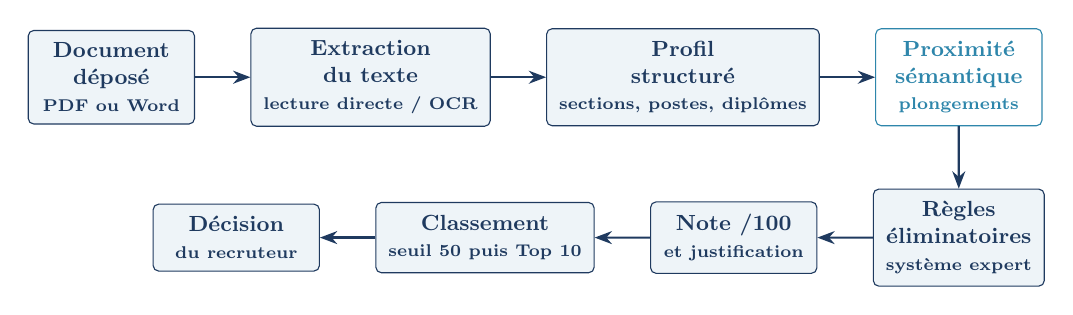
\begin{tikzpicture}[node distance=6mm and 8mm, scale=0.88, transform shape]
    \node[bloc] (cv) {Document\\ déposé\\ \scriptsize PDF ou Word};
    \node[bloc, right=of cv] (extract) {Extraction\\ du texte\\ \scriptsize lecture directe / OCR};
    \node[bloc, right=of extract] (parse) {Profil\\ structuré\\ \scriptsize sections, postes, diplômes};
    \node[blocia, right=of parse] (sem) {Proximité\\ sémantique\\ \scriptsize plongements};
    \node[bloc, below=9mm of sem] (regles) {Règles\\ éliminatoires\\ \scriptsize système expert};
    \node[bloc, left=of regles] (score) {Note /100\\ \scriptsize et justification};
    \node[bloc, left=of score] (classe) {Classement\\ \scriptsize seuil 50 puis Top 10};
    \node[bloc, left=of classe] (dec) {Décision\\ \scriptsize du recruteur};

    \draw[fleche] (cv) -- (extract);
    \draw[fleche] (extract) -- (parse);
    \draw[fleche] (parse) -- (sem);
    \draw[fleche] (sem) -- (regles);
    \draw[fleche] (regles) -- (score);
    \draw[fleche] (score) -- (classe);
    \draw[fleche] (classe) -- (dec);
  \end{tikzpicture}
  \caption{Chaîne de traitement, du dépôt du document à la décision humaine.}
  \label{fig:pipeline}
\end{figure}

\subsection{Lecture du document}
La lecture procède par étapes successives. Le texte est d'abord extrait directement de la couche textuelle du document, méthode rapide et fidèle qui convient à la grande majorité des curriculum vitæ. Lorsque le document ne contient aucun texte exploitable — cas d'un document numérisé, constitué d'images — la reconnaissance optique de caractères prend le relais. Les documents au format Word sont également acceptés, y compris lorsque leur mise en page repose sur des tableaux.

Ce choix d'une cascade plutôt que d'une reconnaissance optique systématique répond à une réalité de terrain : appliquer l'OCR à un document déjà textuel dégraderait la qualité du résultat et multiplierait le temps de traitement.

\subsection{Reconstitution du profil}
Le document est ensuite découpé en sections — expérience, formation, compétences, certifications, langues — à partir d'une liste d'intitulés français et anglais. Cette étape conditionne la fiabilité de tout ce qui suit : une date figurant dans la rubrique « formation » ne doit pas alimenter le calcul de l'expérience professionnelle.

Chaque section est ensuite exploitée pour reconstituer un profil structuré : coordonnées du candidat, postes occupés avec leur intitulé, leur employeur et leurs dates, diplômes avec leur niveau, certifications avec leur organisme, et langues dont le niveau est ramené à l'échelle européenne commune de référence. Le schéma retenu reprend les blocs du format d'échange de fait dans l'industrie du recrutement, ce qui garantit l'interopérabilité du profil produit.

La durée totale d'expérience est calculée à partir des périodes reconstituées, en fusionnant celles qui se chevauchent : deux postes occupés simultanément ne sont pas comptés deux fois.

\subsection{Calcul de la note}
La note finale combine cinq composantes, dont le total est toujours égal à cent afin que les candidatures restent comparables entre elles :

\begin{center}
\small
\begin{tabular}{lcp{7.2cm}}
  \toprule
  \textbf{Composante} & \textbf{Poids} & \textbf{Origine} \\
  \midrule
  Compétences obligatoires & 35 & Référentiel métier appliqué au texte \\
  Compétences souhaitées & 10 & Idem, sans caractère bloquant \\
  Proximité sémantique & 25 & Comparaison du sens du document et de l'offre \\
  Années d'expérience & 20 & Périodes reconstituées \\
  Niveau de diplôme & 10 & Rubrique formation \\
  \bottomrule
\end{tabular}
\end{center}

\vspace{2mm}
\noindent Lorsqu'une composante ne peut être calculée, son poids est reporté sur les compétences obligatoires : le total reste sur cent en toutes circonstances.

Les \textbf{critères éliminatoires} définis par l'offre — expérience minimale, diplôme minimal, compétence indispensable — plafonnent la note à quarante-cinq points et conservent le motif exact du déclassement.

\begin{lstlisting}[caption={Traçage du motif : condition de l'explicabilité de la note.}]
if offre.min_experience_years and experience < offre.min_experience_years:
    eliminatoires.append(
        f"Experience {experience} an(s) < "
        f"{offre.min_experience_years} an(s) requis"
    )
if manquantes:
    eliminatoires.append(
        "Competence(s) obligatoire(s) absente(s) : " + ", ".join(manquantes)
    )
\end{lstlisting}

\subsection{Comportement en cas d'échec}
Une candidature dont le document n'a pas pu être lu n'est jamais perdue ni pénalisée : elle est signalée comme dépourvue de note, distinctement des candidatures écartées, et le recruteur peut relancer l'analyse ou saisir le profil manuellement. Cette distinction évite d'imputer au candidat une insuffisance qui ne serait en réalité qu'un défaut de traitement.

De la même manière, chaque brique technique dispose d'une solution de repli : en l'absence du modèle sémantique, une comparaison lexicale prend le relais ; en l'absence de reconnaissance optique, seuls les documents textuels sont analysés. Le service reste opérationnel dans tous les cas.

% =====================================================================
\section{La plateforme en fonctionnement}
% =====================================================================
Les captures qui suivent proviennent de la plateforme alimentée par un jeu de démonstration : huit offres, dix-huit candidatures et des documents réels traités par la chaîne d'analyse décrite ci-dessus.

\subsection{Espace du recruteur}

\capture{03_recruteur_tableau_de_bord}{Tableau de bord du recruteur. Les indicateurs, l'entonnoir
de conversion et la courbe d'activité sont calculés à partir des données de la base ; le sélecteur
de période recalcule l'ensemble.}{fig:dashboard}

\capture{04_recruteur_candidatures_classees}{Candidatures classées par note décroissante. Les onglets
matérialisent la règle de présélection : liste restreinte, ensemble des candidatures, candidatures
écartées, candidatures sans note.}{fig:candidatures}

\subsection{Explication d'une note}
L'explicabilité constitue l'exigence centrale du projet : le recruteur doit pouvoir comprendre l'origine de chaque note, et le candidat obtenir une justification en cas de refus.

\capture{05_detail_score_profil_ats}{Détail d'une note élevée. Les cinq composantes du calcul sont
détaillées, puis le profil reconstitué depuis le document : coordonnées, durée d'expérience, niveau
de diplôme, parcours professionnel daté.}{fig:detail1}

\capture{06_detail_score_bas_competences}{Suite du panneau : formation, certifications avec leur
organisme, langues avec leur niveau européen, compétences détectées, puis confrontation aux exigences
de l'offre et actions de décision.}{fig:detail2}

\capture{07_candidature_ecartee_motifs}{Candidature écartée. Les motifs exacts sont affichés —
insuffisance d'expérience et absence de compétences obligatoires — et le détail du calcul montre
la part obtenue sur chaque composante. La candidature reste consultable et repêchable.}{fig:ecartee}

\subsection{Assistant et gestion des offres}

\capture{08_assistant_rh_entonnoir}{Assistant conversationnel. Les réponses sont calculées sur les
données réelles de la plateforme et restituées sous forme de tableaux, avec un accès direct à
l'écran concerné.}{fig:assistant}

\capture{09_recruteur_mes_offres}{Gestion des offres publiées, avec le nombre de candidatures reçues
et la note moyenne obtenue par offre.}{fig:offres}

\capture{10_offres_publiees}{Liste des offres telle que présentée aux candidats : localisation,
type de contrat, mode de travail, fourchette de rémunération et compétences attendues.}{fig:offrespub}

\subsection{Espace du candidat}

\capture{02_candidat_suivi_candidatures}{Suivi d'une candidature par le candidat. L'avancement est
présenté par étapes ; la note attribuée par le système n'est volontairement pas exposée, celle-ci
relevant de l'appréciation interne du recruteur.}{fig:candidat}

\subsection{Espace d'administration}

\capture{11_admin_tableau_de_bord}{Tableau de bord de l'administrateur : répartition des comptes,
volumes, et mise en évidence des demandes appelant une décision.}{fig:admin}

\capture{12_admin_validation_recruteurs}{Validation des comptes recruteurs. Publier une offre engage
l'entreprise représentée : chaque demande est donc soumise à l'approbation d'un administrateur, avec
possibilité de refus motivé.}{fig:validation}

\capture{13_admin_roles_permissions}{Matrice des droits. Toute modification s'applique immédiatement
aux utilisateurs du rôle concerné, les permissions étant vérifiées en base à chaque requête.}{fig:roles}

\subsection{Accessibilité}

\capture{14_mode_clair_utilisateurs}{Thème clair. L'ensemble des écrans est déclinable en deux
thèmes, le choix étant conservé d'une session à l'autre et la préférence du système d'exploitation
respectée par défaut.}{fig:clair}

% =====================================================================
\section{Choix structurants et justifications}\label{sec:choix}
% =====================================================================

\subsection{Renoncement à l'apprentissage supervisé}
Le cahier des charges prévoyait un modèle de classification entraîné sur un corpus de curriculum vitæ étiquetés. Ce corpus n'existant pas et sa constitution représentant à elle seule plusieurs jours de travail au résultat incertain, la décision a été prise de fonder le classement sur la combinaison des règles métiers et de la proximité sémantique.

Ce choix est assumé et présente des avantages propres. Un modèle statistique produit une note dont l'origine est difficile à restituer ; l'approche retenue permet au contraire d'expliquer chaque point attribué, ce qui répond directement à l'exigence de transparence du projet et aux obligations réglementaires en matière de décision assistée par algorithme. Le module de score conserve par ailleurs une interface stable : l'ajout ultérieur d'un modèle supervisé ne remettrait pas en cause l'architecture existante.

\subsection{Adoption des conventions professionnelles d'analyse de CV}
L'extraction initialement prévue se limitait à relever des mots-clés. L'expérimentation sur des documents réels a montré les limites de cette approche : sans reconstitution du parcours, il devient impossible de distinguer trois années d'expérience pertinente d'une mention isolée dans une liste de compétences.

L'analyse produit désormais un profil structuré complet, conforme aux pratiques des systèmes professionnels de suivi des candidatures. La distinction entre compétences obligatoires et compétences souhaitées, également issue de ces pratiques, rend le classement nettement plus fidèle aux attentes réelles d'un recruteur.

\subsection{Renforcement de la gouvernance des comptes}
Deux ajouts ont été effectués en cours de sprint. Les comptes recruteurs sont désormais soumis à validation, la publication d'offres engageant l'entreprise représentée. Les suppressions sont devenues réversibles, avec une corbeille permettant la restauration ; la suppression définitive est par ailleurs refusée sur une offre ayant reçu des candidatures, la traçabilité primant sur le nettoyage.

% =====================================================================
\section{Vérification}
% =====================================================================
La couverture de tests a été portée de vingt-cinq à soixante-neuf cas, tous réussis.

\begin{center}
\small
\begin{tabular}{lcc}
  \toprule
  \textbf{Domaine testé} & \textbf{Cas} & \textbf{Résultat} \\
  \midrule
  Authentification et sessions & 6 & \textcolor{vert}{Réussis} \\
  Contrôle d'accès & 3 & \textcolor{vert}{Réussis} \\
  Moteur de notation et règle de présélection & 6 & \textcolor{vert}{Réussis} \\
  Offres, tableau de bord, profil & 5 & \textcolor{vert}{Réussis} \\
  Notifications et cloisonnement & 5 & \textcolor{vert}{Réussis} \\
  Analyse linguistique et sémantique & 14 & \textcolor{vert}{Réussis} \\
  Reconstitution du profil structuré & 16 & \textcolor{vert}{Réussis} \\
  Validation des comptes et corbeille & 14 & \textcolor{vert}{Réussis} \\
  \midrule
  \textbf{Total} & \textbf{69} & \textcolor{vert}{\textbf{100 \%}} \\
  \bottomrule
\end{tabular}
\end{center}

\vspace{2mm}
\noindent Au-delà des tests unitaires, la cohérence du classement a été contrôlée sur un ensemble de profils dont la qualité attendue était connue à l'avance. Les notes obtenues respectent l'ordre attendu, avec un écart net entre les catégories, ce qui confirme le pouvoir discriminant du moteur.

\begin{center}
\small
\begin{tabular}{lcc}
  \toprule
  \textbf{Qualité attendue du profil} & \textbf{Note moyenne} & \textbf{Effectif} \\
  \midrule
  Profil très adapté & 88 / 100 & 6 \\
  Profil adapté & 76 / 100 & 5 \\
  Profil partiellement adapté & 45 / 100 & 3 \\
  Profil non adapté & 37 / 100 & 2 \\
  \bottomrule
\end{tabular}
\end{center}

% =====================================================================
\section{Planification}
% =====================================================================

\begin{center}
\small
\begin{tabular}{clcc}
  \toprule
  \textbf{Sprint} & \textbf{Contenu} & \textbf{Période} & \textbf{Durée} \\
  \midrule
  1 & Socle technique, base de données, sécurité & 06/07 -- 15/07 & 10 jours \\
  2 & Interface, parcours métier, notifications & 16/07 -- 27/07 & 12 jours \\
  3 & Analyse des CV, classement explicable & 28/07 -- 06/08 & 10 jours \\
  4 & Décisionnel, indicateurs, finalisation & 07/08 -- 16/08 & 10 jours \\
  \bottomrule
\end{tabular}
\end{center}

\begin{figure}[H]
  \centering
  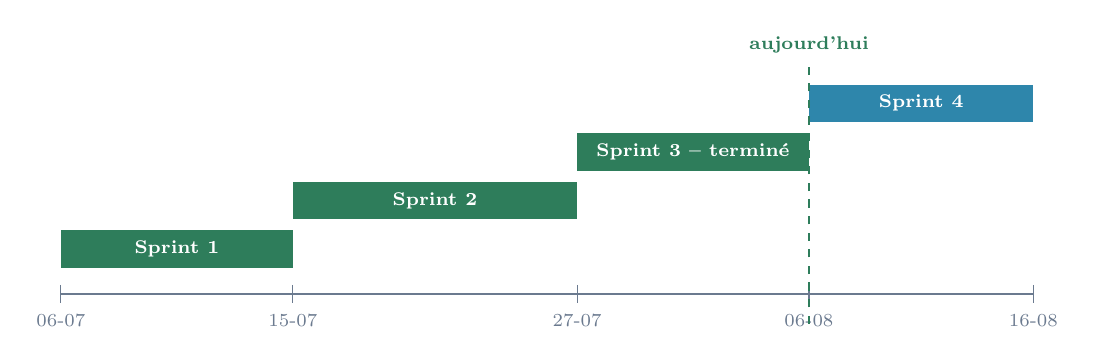
\begin{tikzpicture}[scale=0.95, transform shape]
    \draw[gris, thick] (0,0) -- (13,0);
    \foreach \x/\lab in {0/06-07, 3.1/15-07, 6.9/27-07, 10/06-08, 13/16-08} {
      \draw[gris] (\x, 0.12) -- (\x, -0.12);
      \node[font=\scriptsize, color=gris, below] at (\x, -0.15) {\lab};
    }
    \fill[vert] (0, 0.35) rectangle (3.1, 0.85);
    \node[white, font=\scriptsize\bfseries] at (1.55, 0.6) {Sprint 1};
    \fill[vert] (3.1, 1.0) rectangle (6.9, 1.5);
    \node[white, font=\scriptsize\bfseries] at (5.0, 1.25) {Sprint 2};
    \fill[vert] (6.9, 1.65) rectangle (10, 2.15);
    \node[white, font=\scriptsize\bfseries] at (8.45, 1.9) {Sprint 3 -- terminé};
    \fill[accent] (10, 2.3) rectangle (13, 2.8);
    \node[white, font=\scriptsize\bfseries] at (11.5, 2.55) {Sprint 4};
    \draw[dashed, thick, color=vert] (10, -0.4) -- (10, 3.1);
    \node[font=\scriptsize\bfseries, color=vert, above] at (10, 3.1) {aujourd'hui};
  \end{tikzpicture}
  \caption{Avancement du projet à la clôture du Sprint 3.}
  \label{fig:gantt3}
\end{figure}

\subsection{Contenu du Sprint 4}
Les travaux restants portent sur la restitution décisionnelle et la finalisation :
\begin{itemize}[leftmargin=1.5em, nosep]
  \item rapports décisionnels sous Power BI, connectés à la base de données ;
  \item mesure des indicateurs de performance annoncés au cahier des charges ;
  \item vérification de l'absence de corrélation entre les notes et des attributs non pertinents ;
  \item tests de bout en bout des parcours critiques ;
  \item documentation d'exploitation et préparation de la soutenance.
\end{itemize}

% =====================================================================
\section{Risques et mesures}
% =====================================================================

\begin{center}
\small
\begin{tabular}{p{4.6cm}cp{7.4cm}}
  \toprule
  \textbf{Risque} & \textbf{Criticité} & \textbf{Mesure retenue} \\
  \midrule
  Diversité des mises en page de curriculum vitæ & Moyenne & Découpage en sections avec mode de repli ; toute candidature illisible reste traitable manuellement. \\[1mm]
  Absence de modèle supervisé & Moyenne & Choix assumé et documenté ; l'explicabilité du dispositif retenu compense l'absence d'apprentissage statistique. \\[1mm]
  Densité du Sprint 4 & Moyenne & Priorisation : les indicateurs et le décisionnel priment sur la mise en ligne distante, remplaçable par une démonstration conteneurisée. \\[1mm]
  Coût des services externes & Faible & Sélection exclusive d'outils gratuits ou en licence libre pour l'ensemble de la chaîne. \\
  \bottomrule
\end{tabular}
\end{center}

% =====================================================================
\section{Conclusion}
% =====================================================================
Le Sprint~3 est clôturé conformément au calendrier. La plateforme remplit désormais sa fonction première : un curriculum vitæ déposé est lu automatiquement, quel que soit son format, décomposé en un profil structuré, confronté aux exigences de l'offre, et noté selon un calcul dont chaque élément est restitué au recruteur.

Le renoncement à l'apprentissage supervisé, décidé en début de sprint, s'est révélé bénéfique au-delà du seul gain de temps : il a conduit à concentrer l'effort sur la qualité de l'extraction et sur la transparence du classement, qui constituent la véritable valeur du dispositif. Un système capable de justifier chaque décision répond mieux aux besoins d'un recruteur — et aux obligations réglementaires — qu'un modèle statistique dont les résultats resteraient inexplicables.

Le Sprint~4 sera consacré à la restitution décisionnelle, à la mesure des indicateurs annoncés et à la préparation de la livraison finale.

\end{document}
